\documentclass{article}

\usepackage{listings}
\usepackage{graphicx}
\usepackage{amsmath}
\usepackage[dvipsnames]{xcolor}
\usepackage{stackengine}

\newcommand{\flecha}[2] {
    \!\!$\overset{\text{#1}}{\overset{\downarrow}{\text{#2}}}$\!\!
}

\usepackage{geometry}
 \geometry{
 a4paper,
 total={170mm,257mm},
 left=20mm,
 top=20mm,
 }

 \definecolor{codegreen}{rgb}{0,0.6,0}
 \definecolor{codegray}{rgb}{0.5,0.5,0.5}
 \definecolor{codepurple}{rgb}{0.58,0,0.82}
 \definecolor{backcolour}{rgb}{0.95,0.95,0.92}
 
 \lstdefinestyle{mystyle}{
     backgroundcolor=\color{backcolour},   
     commentstyle=\color{codegreen},
     keywordstyle=\color{magenta},
     numberstyle=\tiny\color{codegray},
     stringstyle=\color{codepurple},
     basicstyle=\ttfamily\footnotesize,
     breakatwhitespace=false,         
     breaklines=true,                 
     captionpos=b,                    
     keepspaces=true,                 
     numbers=left,                    
     numbersep=5pt,                  
     showspaces=false,                
     showstringspaces=false,
     showtabs=false,                  
     tabsize=2
 }

 \lstset{style=mystyle}

\graphicspath{{./Imagenes/}}

\begin{document}
\section*{Explicación del algoritmo}

\subsection*{Idea inicial}
El objetivo del programa es el de poder identificar las palabras a espaciar en una única lectura del texto de entrada.
Para ello es necesario poder rastrear multiples palabras del diccionario al mismo tiempo.

Para lograr esto se guardan todas las palabras en un árbol general, cada nodo del árbol va a representar un posible
prefijo de una palabra del diccionario. Las aristas del árbol se etiquetan con un carácter del alfabeto, de modo que si
un nodo A con la palabra $p$ esta conectado a otro nodo B mediante una arista con el carácter $c$, entonces la palabra
que contiene el nodo B es $p+c$.

Por ejemplo el árbol para el diccionario ["quien", "deposito", "dolar", "dolares", "es", "recibira"] es:

\begin{center}
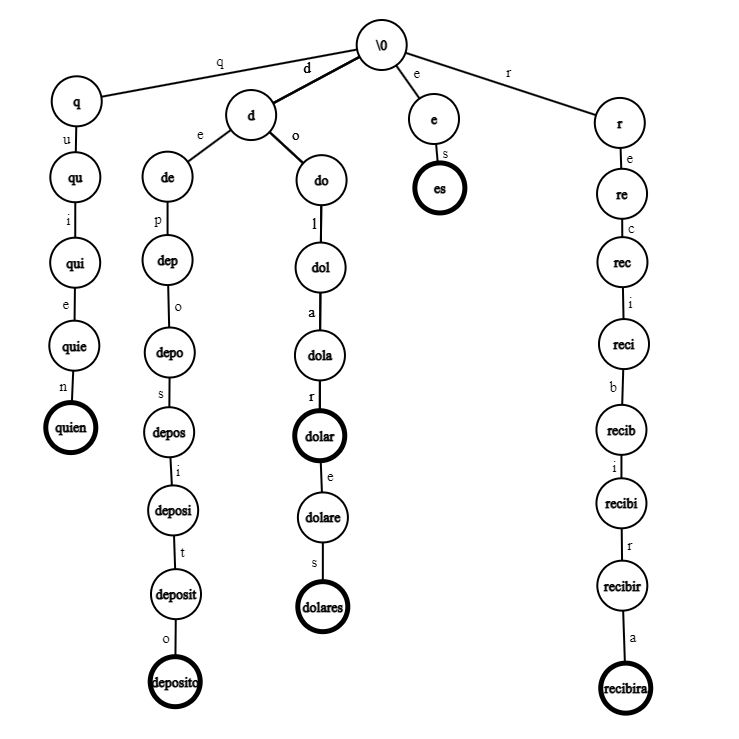
\includegraphics[scale=0.3]{trie1.png}
\end{center}

Los nodos a su vez tienen que indicar si el prefijo representa una palabra que esta en el diccionario, en el gráfico
eso queda representado por un circulo de un color mas fuerte.

Usando este árbol, se puede analizar el string como sigue. Se inicializan dos iteradores i,j al inicio de la palabra a analizar,
en cada paso se mueve el iterador j y se recorre el árbol en la arista correspondiente. Si en algún momento se llega a un nodo
con una palabra del diccionario se guarda la posición actual en una variable k(esta variable se sobrescribe si se encuentra otra
palabra mas grande). Cuando se llega a un punto en el que no se puede seguir por el árbol, la palabra encontrada es el substring
[i:k]. Después se avanza el iterador i hasta k+1(hasta i+1 en el caso en que no se encontró una palabra) y se vuelve a la raíz del 
árbol para continuar el análisis.

Asi para el diccionario de ejemplo, la palabra "dosdolares" se espacia de esta forma:

\begin{center}
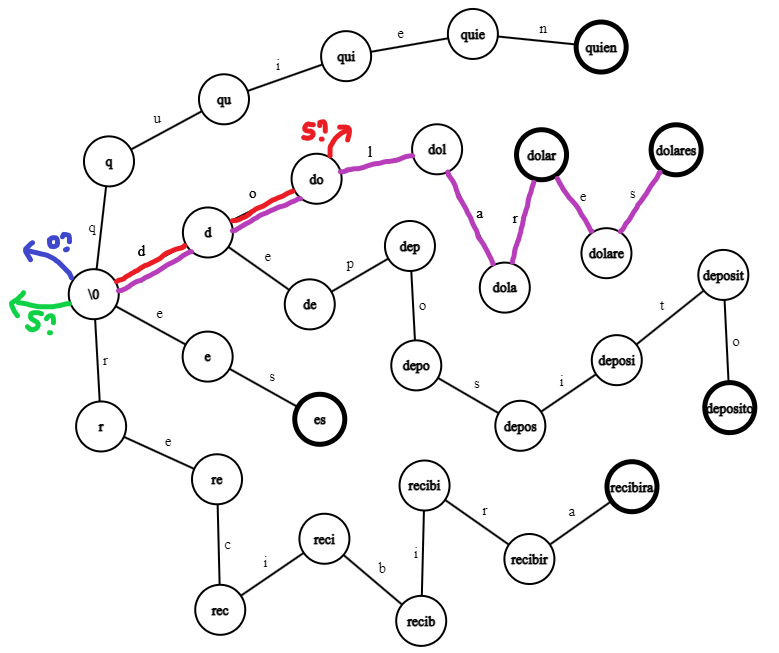
\includegraphics[scale=0.4]{ejemplo_trie1.png}
\end{center}

{\color{red} \underline{\textbf{Primer recorrido 1:}}} \flecha{i,j}{d}osdolares $\rightarrow$ \flecha{i}d\flecha{j}osdolares $\rightarrow$ \flecha{i}do\flecha{j}sdolares $\rightarrow$ {\color{red} \textbf X}

El nodo "do" no tiene una arista con el carácter 's', como no se puede seguir vuelvo a la raíz y avanzo i un lugar para adelante.

{\color{blue} \underline{\textbf{Segundo recorrido 2:}}} d\flecha{i,j}osdolares $\rightarrow$ {\color{red} \textbf X}

La raíz no tiene una arista con el carácter 'o', como no se puede seguir, paso al carácter siguiente.

{\color{Green} \underline{\textbf{Tercer recorrido 3:}}} do\flecha{i,j}sdolares $\rightarrow$ {\color{red} \textbf X}

La raíz no tiene una arista con el carácter 's', como no se puede seguir, paso al carácter siguiente.

{\color{violet} \underline{\textbf{Cuarto recorrido 4:}}} dos\flecha{i,j}dolares $\rightarrow$ dos\flecha{i}d\flecha{j}olares $\rightarrow$ dos\flecha i do\flecha j lares
$\rightarrow$ dos\flecha i dol\flecha j ares $\rightarrow$ dos\flecha i dola\flecha j res

Se encontró la palabra "dolar", se marca con una flecha k

dos\flecha i dola\flecha k r\flecha j es $\rightarrow$ dos\flecha i dola\flecha k re\flecha j s $\rightarrow$ {\color{red}\textbf{X}}

Se encontró la palabra "dolares", se marca con una flecha k:

dos\flecha i dolare\flecha k s $\rightarrow$ {\color{red}\textbf{X}}

No se puede seguir porque se termino de leer el string, la palabra mas larga encontrada fue "dolares":

La salida final del programa es: "dolares"

Esta idea no es lo suficientemente optima ya que el indice j tiene que retroceder junto al indice i para analizar caracteres que
ya fueron revisados. Esto hace que en algunos casos el algoritmo realiza $N^2$ operaciones, donde $N$ es el largo del string. Es el caso
de la palabra "cinco" con el diccionario ["cincos","incos","ncos","cos","os","s"]

Para poder evitar esto, es necesario agregar información adicional en el árbol.

\subsection*{Optimización: transiciones de falla}

La idea de la optimización es que si no se puede seguir recorriendo el árbol desde un nodo $B$, en vez de volver a la raíz y recorrer desde ahi hasta un cierto nodo $A$,
se salte directamente del nodo $B$ al nodo $A$. De esta manera se "reciclan" los caracteres que había entre $i$ y $j$ en vez leerlos nuevamente.

A la transición que permite conectar el nodo $B$ con el nodo $A$ la llamo \textbf{transición de falla}.

Dado que es posible llegar desde el nodo raíz hasta el nodo $A$ usando uno o mas de los caracteres finales de la palabra de $B$. El prefijo que representa $A$ es a su vez
un sufijo propio de $B$. Además, si tiene como ancestro a una palabra aceptada del diccionario $x$, entonces el prefijo al que apunta
su transición de falla no puede tener intersección con $x$(por ejemplo, en el diccionario ["dolares","dolar"
,"eco","arepa"] el nodo con el prefijo "dolare" de la palabra "dolares" podria
apuntar al nodo con el prefijo "are" de la palabra "arepa", pero como los caracteres 'a' y 'r' ya se
usaron para formar la palabra "dolar" esto no es posible, asi que la transición de falla termina apuntando
al prefijo "e" de la palabra "eco" ).

En particular, $A$ contiene al sufijo propio mas grande de $B$ que cumple con la restricción mencionada arriba.

Estas serian algunas de las transiciones de falla para el árbol de ejemplo. Las aristas en rojo marcan las transiciones de falla. Dado que pueden ser muchas y el grafico
puede volverse engorroso, los nodos que no tienen aristas rojas tienen su transición de falla apuntando a la raíz:

\begin{center}
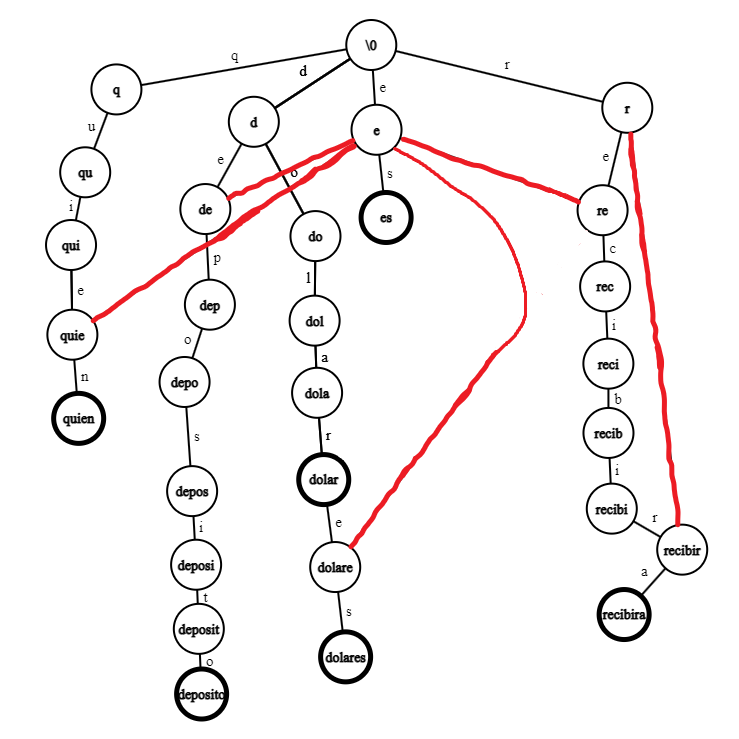
\includegraphics[scale=0.4]{Imagenes/trie1_transiciones_falla.png}
\end{center}

De esta forma, si en un cierto punto se quiere leer el carácter 'x' y el nodo actual no posee una arista con dicho carácter,
se sigue la transición de falla y se revisa si es posible seguir desde ahi con el carácter 'x', en caso contrario se sigue la transición de falla del nodo al que recién se llego y se repite el proceso.

Eventualmente las transiciones de falla terminan en la raíz, si se llega hasta la raíz y no es posible seguir con el carácter 'x', entonces se descarta el carácter y se sigue leyendo el string.

Un codigo del procedimiento de arriba puede ser este
\begin{lstlisting}[language=C]
    Nodo seguirArista(Nodo n, char c) {
        
        // Si el nodo n no tiene una arista con el caracter c entonces salto por
        // las transiciones de falla, si en algun punto llego a la raiz entonces paro.
        while(n != raiz && !sePuedeSeguir(n,c))
            n = n.transicionDeFalla;
        
        // Si el nodo en el que termine tiene una arista con el caracter s, entonces
        // la sigo
        if(sePuedeSeguir(n,s))
            n = n.hijos[s];
        
        return n;
    }
\end{lstlisting}

Con las transiciones de falla incluidas, el árbol ya puede usarse como si fuera un Autómata de Estado Finito(de hecho, asi es como se lo llama en el código).

Para el ejemplo de la palabra "dosdolares", con el diccionario ["dolar","dolares"] el espaciado se calcularía asi:

\begin{center}
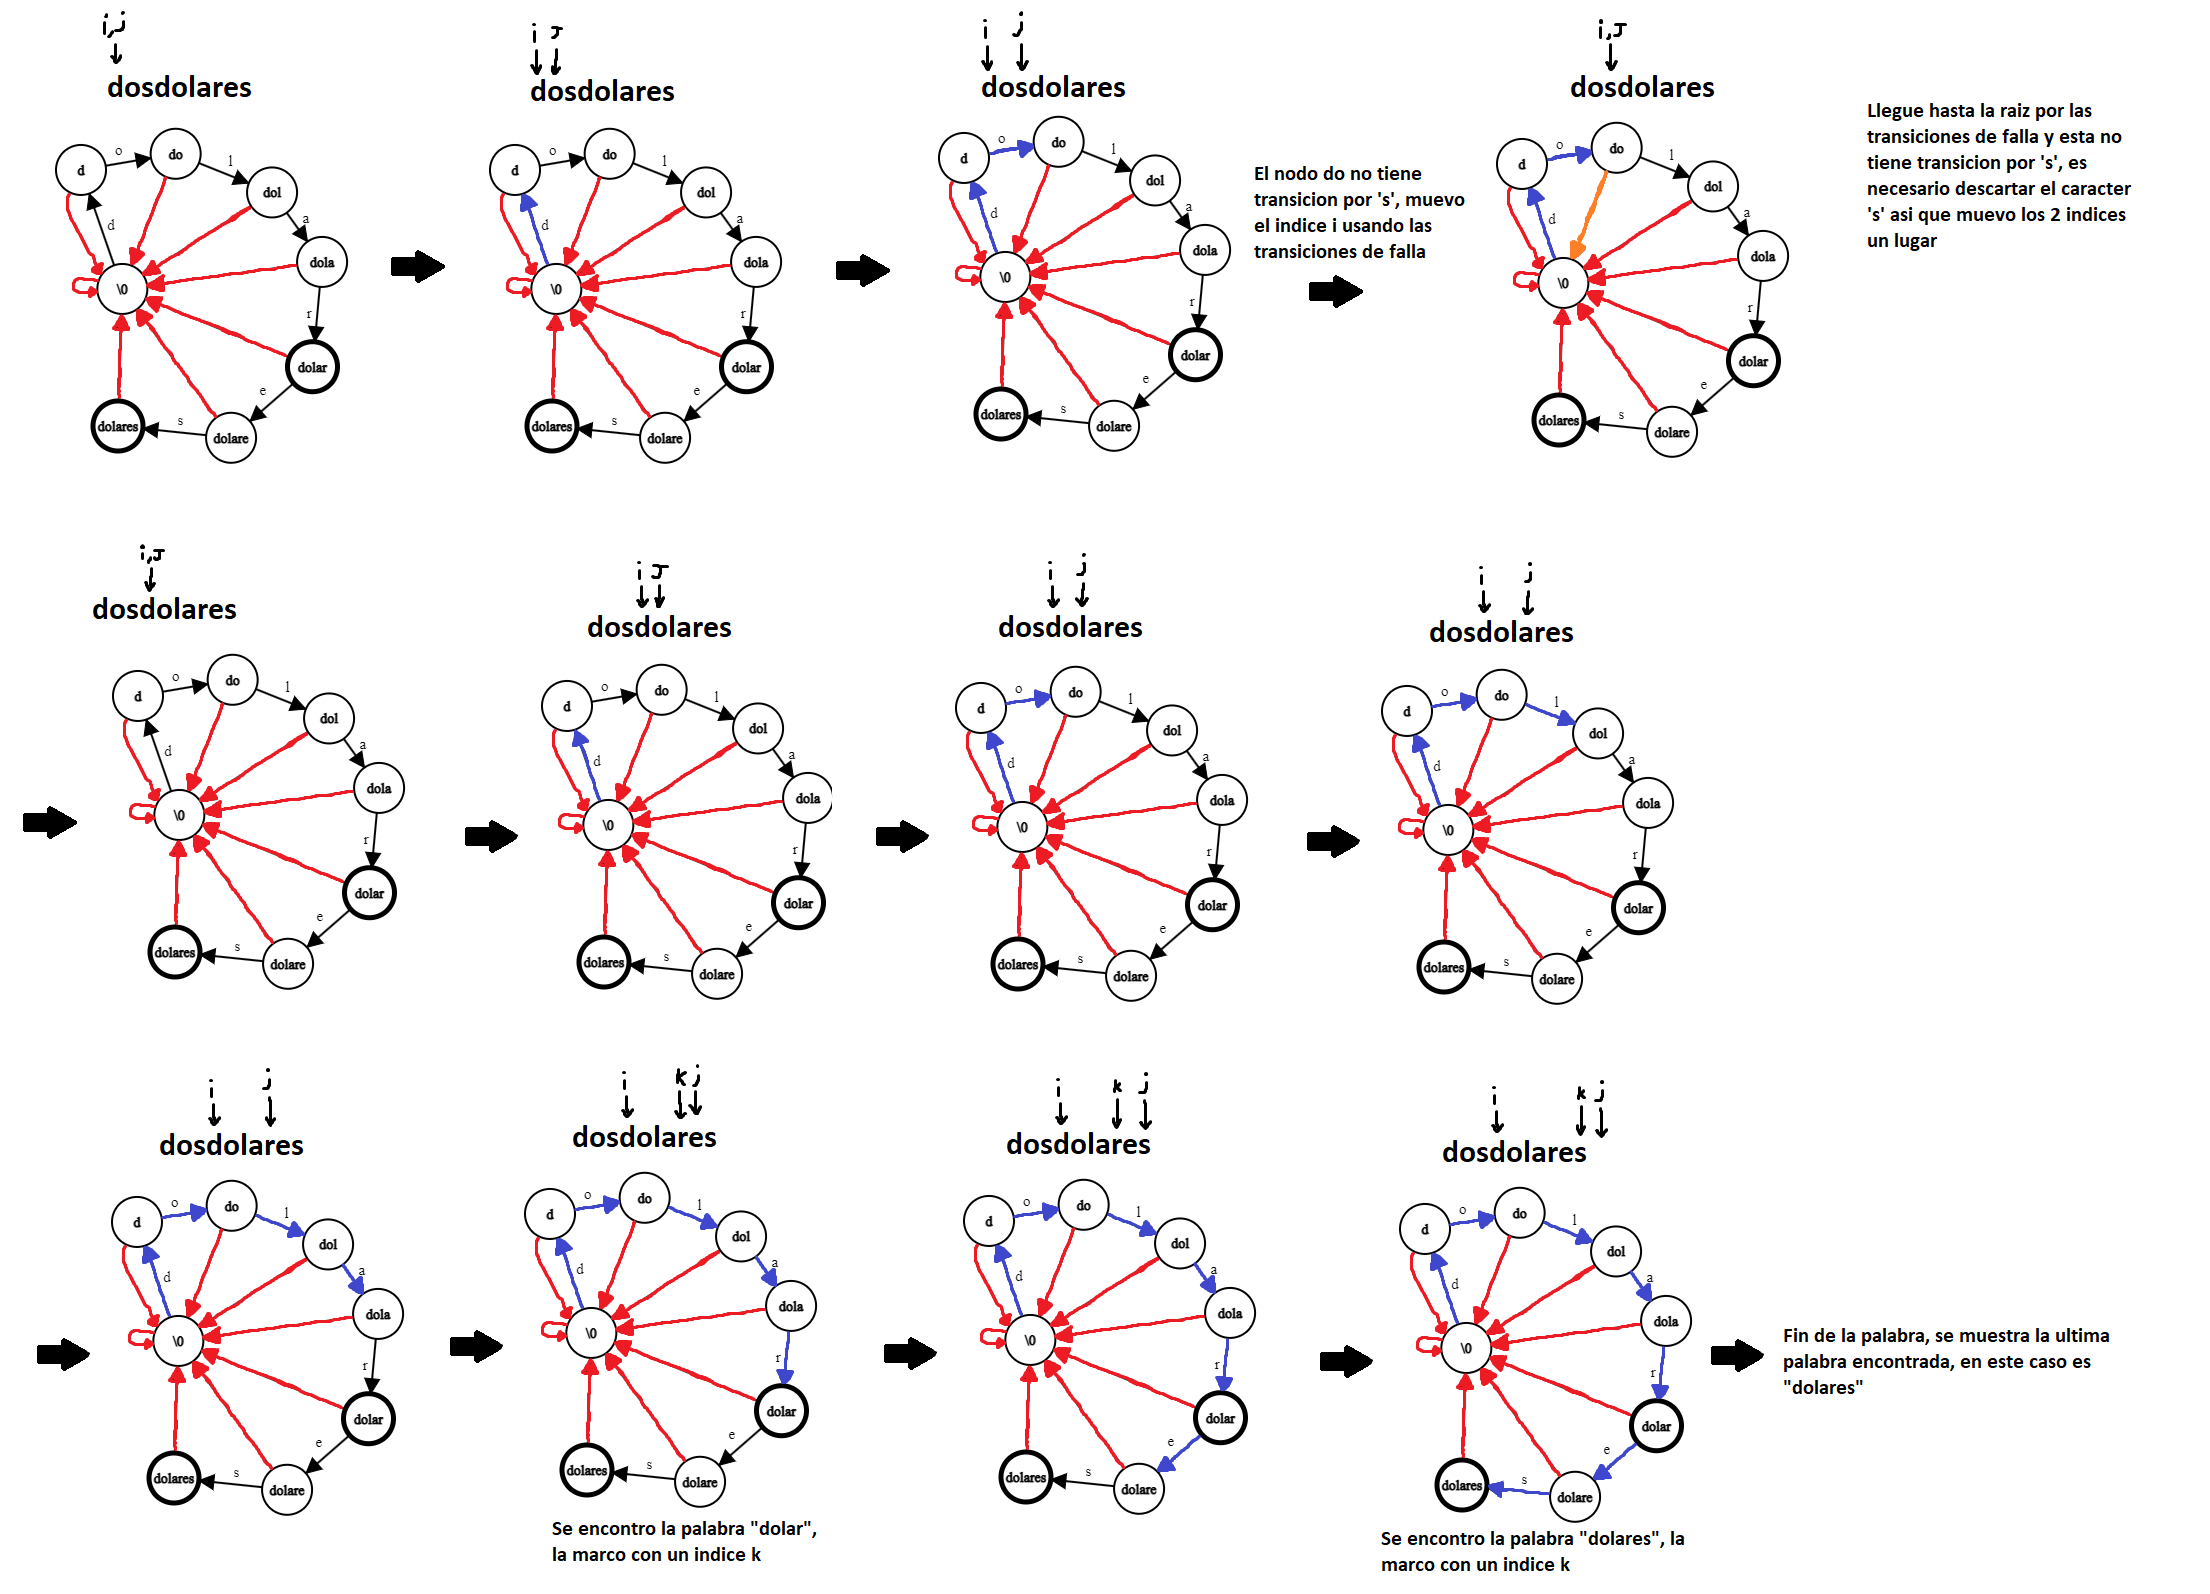
\includegraphics[scale=0.3]{Imagenes/automata_falla_ejemplo_dosdolares.png}
\end{center}

Suponiendo que el autómata ya esta construido, espaciar una frase tiene una complejidad $O(N)$ donde $N$ es el largo de la frase a espaciar.
Esto es asi porque cada letra de la frase es visitada una sola vez por los indices $i$ y $j$ que avanzan linealmente.

\newpage

Sin embargo el algoritmo tiene errores, por ejemplo, para la palabra "dola" y el diccionario ["dolar","ol"] el algoritmo es como sigue:

\begin{center}
    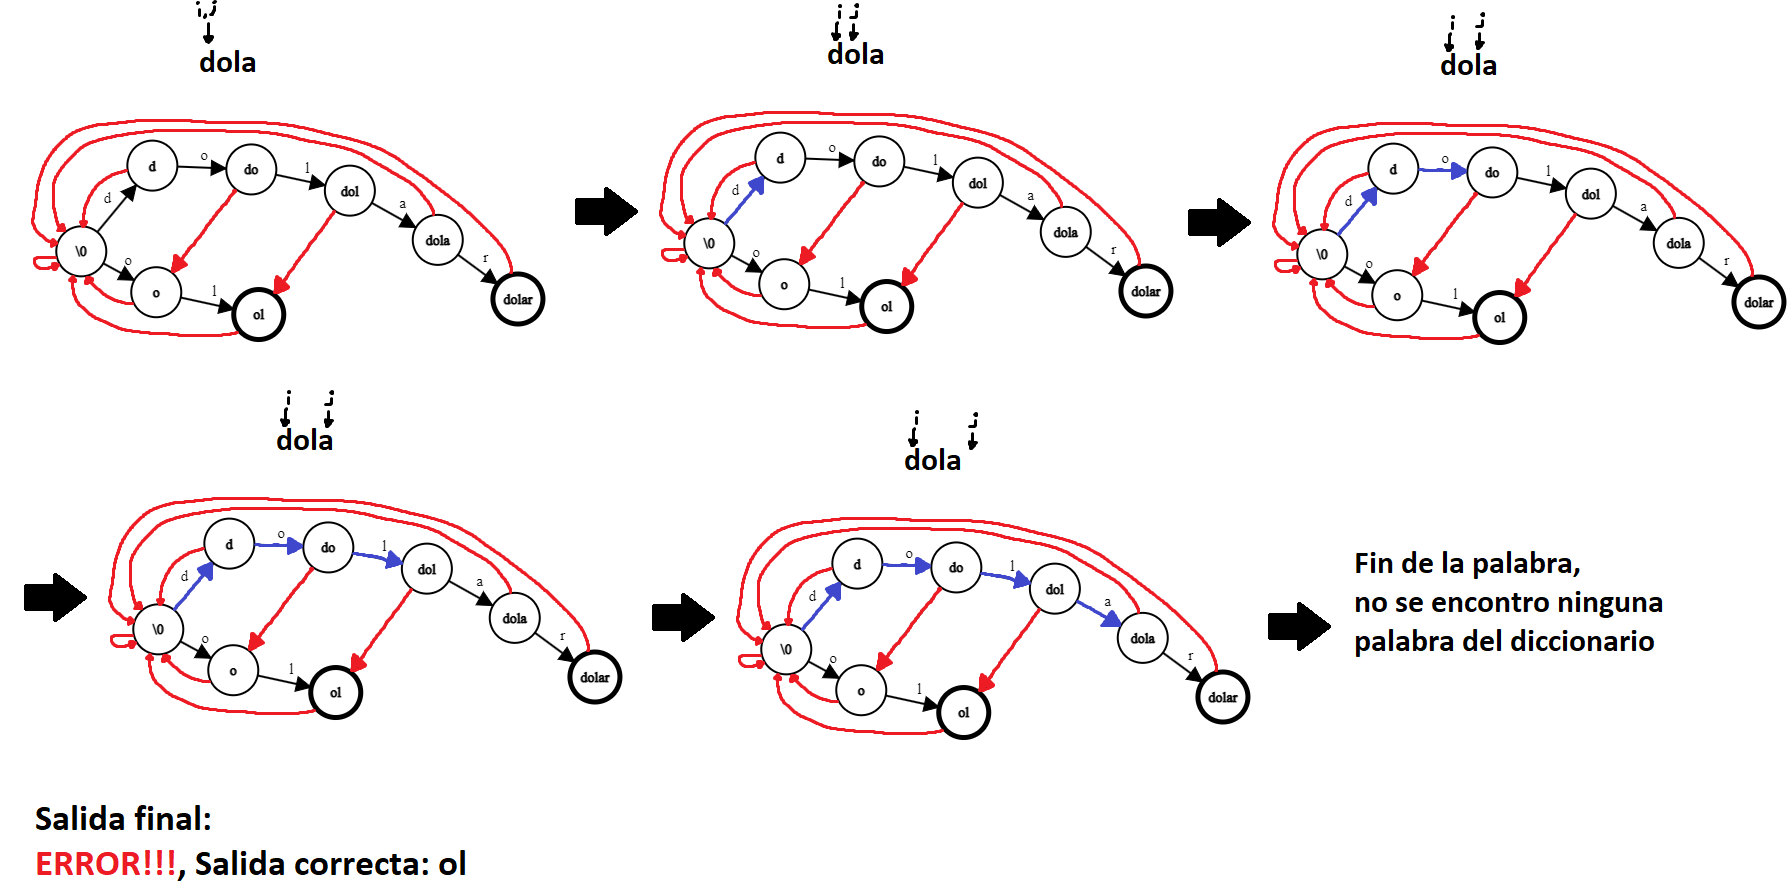
\includegraphics[scale=0.3]{Imagenes/automata_falla_ejemplo_dola.png}
\end{center}

\subsection*{Solución: transiciones de salida}

Un primer intento de solucionar este problema es que cuando se llega a un estado cualquiera, se empiezan a recorrer las transiciones de falla
hasta la raíz, si en el camino se encuentra un estado de aceptación entonces se registra de alguna manera que una palabra se encontró.
Como la distancia entre 2 estados de aceptación unidos por transiciones de falla puede ser bastante grande, esta opción puede resultar ineficiente.

Para optimizar esta solución se pueden añadir nuevas transiciones al autómata, las \textbf{transiciones de salida}. Las transiciones de salida apuntaran a un nodo es de aceptación
y esta unido al nodo actual por una o mas transiciones de falla. Para el ejemplo anterior, la transición de salida del nodo con la palabra "dol" apuntaría al nodo con la palabra "ol" y
todos los nodos restantes quedan sin transición de salida.

De esta manera, cuando se llega a un nodo cualquiera, se recorren las transiciones de salida y se registran las palabras encontradas en el camino. Si bien el método es bastante similar al anterior, este
es mas eficiente ya que solo visita los nodos de aceptación y se "saltea" los nodos que no son de aceptación.

El automata completo para el diccionario ["dolar","ol"] queda como sigue:

\begin{center}
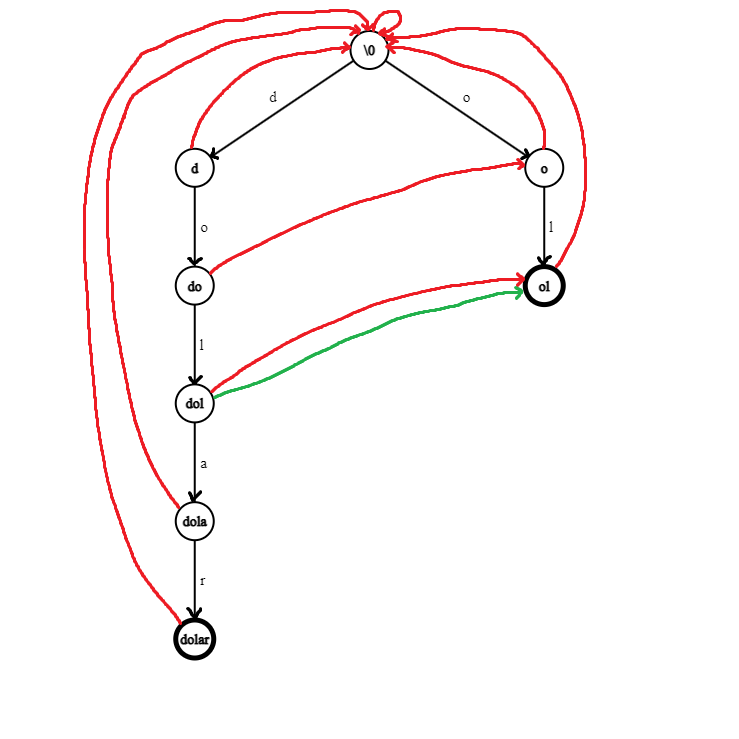
\includegraphics[scale=0.3]{Imagenes/automata_completo_dolar_ol.png}
\end{center}

\subsection*{Espaciado de las palabras}

Ahora el algoritmo tiene que poder lidiar con palabras aceptadas que están entre medio de los indicies $i$ y $j$. Asi que en lugar de guardar un indice $k$ hay que almacenar intervalos enteros $(l,r)$ de palabras
aceptadas y cuando el índice $i$ avance los intervalos se irán procesando. Los intervalos que se procesaran primero serán aquellos que tengan menor coordenada inicial y mayor longitud.

Un posible código del algoritmo para procesar intervalos es el siguiente:

\begin{lstlisting}[language=C]
        // i, j son los indices
        // string es el string que estoy espaciando
        // S = Estructura donde se guardan los intervalos
        
        /*
            Los intervalos tienen la siguiente forma:
            typedef struct {
                int inicio;
                int final;
            } Intervalo;
        */

        for(int k=0;k < letrasADescartar; k++)
        {
            // Si no hay intervalos para procesar, el indice i avanza
            if(!hay_intervalos(S))
            {
                i++;
                k++;
            }
            else
            {
                Intervalo inter = obtener_primer_intervalo(S);

                // Si faltan letras para llegar a la palabra a espaciar,
                // avanzo los indices sin imprimir nada
                while(i<inter.primero && k<letrasADescartar)
                {
                    i++;
                    k++;
                }
                // Proceso el intervalo, mostrando todas las letras que representa
                while(i<=inter.final)
                {
                    i++;
                    k++;
                    printf("%c",string[i])
                }

                // Imprimo un espacio
                printf(" ");

                // Bajo en uno el indice k para que despues el for lo reestablezca
                k--;
            }

            // Si algun intervalo se queda atras del indice i entonces hay que eliminarlo
            while(hayIntervalos(S) && obtener_primer_intervalo(S).inicio < i)
                elminar_primer_intervalo(S)
        }
\end{lstlisting}

La estructura S usada en el código cumple las especificaciones de una \textbf{cola de prioridad}.

En el caso del código del programa, la frase no se guarda completamente en memoria sino que solamente se almacena la parte que se
esta revisando(en el caso del ejemplo, seria el pedazo de la frase representado por los indices $i$ y $j$) asi que la implementación difiere un poco.

La parte representada por los indices $i$ y $j$ se almacena en una cola de caracteres. Cuando el indice $i$ avanza se saca un elemento y cuando el indice $j$ avanza
se mete un elemento. Asi que para saber en que parte de la frase esta, el programa se guarda en una variable entera el indice del primer carácter de la cola(en el código
se llama indice). Este enfoque evita el tener que cargar toda la frase en memoria, por lo que resulta mas eficiente.

Ademas, los espacios se imprimen antes de mostrar el string(para que no quede un espacio suelto al final). Asi que también se tiene una variable booleana que indica si hay que
imprimir un espacio o no.

El código para procesar los caracteres queda asi:

\begin{lstlisting}[language=C]

    // cola: la cola de caracteres antes nombrada
    // colaIntervalos: cola de prioridad de intervalos enteros
    // archivoSalida: archivo donde se imprimen los caracteres
    // imprimirEspacio: indica si hace falta imprimir un espacio o no
    // indice: indice de la primera letra de la cola en la frase a espaciar
    int ultimoFin = -1;
    for (int i = 0; i < letrasADescartar && !cola_empty(cola); i++)
    {
        // Si no hay intervalos para procesar, se descartan caracteres
        if (cola_intervalos_vacia(*colaIntervalos))
            cola = cola_pop(cola);
        else
        {
            // Obtengo el intervalo a procesar
            Intervalo inter = cola_intervalos_obtener_primero(*colaIntervalos);
            int seProcesaranLetras = inter.inicio <= letrasADescartar + indice;

            // Si se procesaran letras, entonces hay que imprimir un espacio si es necesario
            if (seProcesaranLetras)
            {
                if (imprimirEspacio)
                    fputc(' ', archivoSalida);
                // Se va a imprimir una palabra, todas las palabras siguientes tienen que tener un espacio
                imprimirEspacio = 1;
            }

            // Descarto los caracteres que no se van a procesar
            while (indice + i < inter.inicio && i < letrasADescartar && !cola_empty(cola))
            {
                cola = cola_pop(cola);
                i++;
            }

            // Los caracteres que se van a procesar se imprimen
            if (seProcesaranLetras)
            {
                while (indice + i <= inter.final && !cola_empty(cola))
                {
                    fputc(cola_front(cola), archivoSalida);
                    cola = cola_pop(cola);
                    i++;
                }
                ultimoFin = indice + i - 1;
                i--;
            }
        }
        // Puede haber intervalos que se solapen con la ultima palabra procesada, de ser asi, tienen que ser eliminados de la cola de prioridad
        while (!cola_intervalos_vacia(colaIntervalos) && (cola_intervalos_obtener_primero(colaIntervalos).inicio <= indice || ultimoFin >= cola_intervalos_obtener_primero(colaIntervalos).inicio))
            colaIntervalos = cola_intervalos_eliminar_primero(colaIntervalos);
    }
\end{lstlisting}

Y para leer las palabras de la frase el código queda como sigue:

\begin{lstlisting}[language=C]
    // estadoInicial es el estadoInicial del automata
    // De archivoEntrada se sacan las frases a espaciar
    // En archivoSalida se guardan las frases ya espaciadas

    // Uso una cola para guardar temporalmente los caracteres que pueden formar una palabra a espaciar
    Cola cola = cola_crear(copy_char, destruir_char);

    // heap_intervalos es usado como una cola de prioridad, permite obtener los intervalos que tienen menor coordenada
    // inicial y que tienen mayor largo
    colaIntervalos colaIntervalos = cola_intervalos_crear(10);

    // Inicialmente, el estado actual es el inicial
    EstadoAutomata* estadoActual = estadoInicial;

    // Si esta variable tiene valor 1, se imprimira un espacio antes de mostrar una palabra encontrada
    // Cuando se encuentra e imprime la primer palabra, su valor cambia a 1. De esta forma la segunda palabra en adelante
    // queda con un espacio al inicio y todas las palabras quedan espaciadas
    int seEncontroUnaPalabra = 0;

    // Indice de la letra actual en la palabra a analizar
    int indice = 0;

    // Empiezo a leer el archivo de entrada
    while (!feof(archivoEntrada))
    {
        char c = fgetc(archivoEntrada);

        // Solo se permiten caracteres de fin de linea/archivo o letras del abecedario
        if (!(c == '\r' || c == '\n' || c == EOF || ('a' <= tolower(c) && tolower(c) <= 'z')))
        {
            fprintf(stderr, "CARACTER INVALIDO %c(%d)\n", c, c);
            assert(0);
        }

        // Si llegue al fin de una linea o al fin del archivo, hay que consumir
        // los caracteres sobrantes y reinciar el automata a como estaba inicialmente
        if (c == '\r' || c == '\n' || c == EOF)
        {
            if (c == '\r')
                fgetc(archivoEntrada);
            
            // Codigo para procesar caracteres...
            
                // Imprimo un caracter de fin de linea si es necesario
            if (c != EOF)
                fputc('\n', archivoSalida);
            // Dejo el automata a como estaba inicialmente
            seEncontroUnaPalabra = 0;
            estadoActual = estadoInicial;
            indice = 0;
            assert(indice == 0);
        }
        // Si no llegue al fin de linea o al fin del archivo entonces proceso
        // el caracter
        else
        {
            // Meto el caracter en la cola y aumento el indice
            cola = cola_push(cola, &c);


            // Para saber si hay que descartar caracteres, me fijo en el largo de los prefijos
            // del automata, si el prefijo que estoy viendo no aumento en una unidad respecto al
            // anterior, es porque hay que descartar caracteres y recuperarse de errores.

            // Sigo la transicion correspondiente al caracter leido.
            int prevLargo = estadoActual->largoPrefijo;
            estadoActual = automata_seguir_transicion(estadoActual, tolower(c));

            // Si hay letras a descartar es necesario recuperarse de errores
            int letrasADescartar = prevLargo - estadoActual->largoPrefijo + 1;

            // Proceso los caracteres si es necesario
            // Codigo para procesar caracteres...

            indice += letrasADescartar;

            // Se llego a un estado de aceptacion, meto el intervalo que representa la palabra actual a la cola de intervalos
            if (estadoActual->palabraAceptada)
                colaIntervalos = cola_intervalos_insertar(colaIntervalos, intervalo_crear(indice, indice + estadoActual->largoPrefijo - 1));
            // Si existe algun sufijo propio de la palabra actual que esta en el diccionario, se inserta su intervalo correspondiente en la cola
            // de prioridad, puedo acceder a estos sufijos usando las transiciones de salida
            for (EstadoAutomata *estado_salida = estadoActual->transicionDeSalida; estado_salida != NULL; estado_salida = estado_salida->transicionDeSalida)
                colaIntervalos = cola_intervalos_insertar(colaIntervalos, intervalo_crear(indice + estadoActual->largoPrefijo - estado_salida->largoPrefijo, indice + estadoActual->largoPrefijo - 1));
        }
    }
    cola_intervalos_destruir(colaIntervalos);
    cola_destroy(cola);
\end{lstlisting}

\subsection*{Complejidad}

El siguiente análisis no tiene en cuenta el costo en tiempo y memoria de construir el automata. Dicho costo se explica en la siguiente sección. 

\subsubsection*{Complejidad temporal}
El algoritmo para espaciar las palabras lee y descarta cada caracter exactamente una vez y luego tiene que usar la cola de prioridad para procesar las palabras encontradas. La complejidad seria en total
$O(N)+f(Z)$, donde $N$ es el string a procesar y $Z$ son la cantidad de apariciones de las palabras a espaciar. $f(Z)$ depende de la implementación
de la cola de prioridad de intervalos, mas específicamente $f(Z) = O(Z \cdot (\text{Costo de Insertar} + \text{Costo de obtener primero} + \text{Costo de eliminar primero}))$.

Se tuvieron en cuenta 2 posibles implementaciones de una cola de prioridad de intervalos:

\begin{description}
    \item[Usar un heap de intervalos enteros:] La idea es mantener el elemento con mayor prioridad en la raíz del heap e ir insertando y eliminando elementos
    del mismo mientras se mantiene la invariante heap(todo nodo siempre tiene mas prioridad que sus hijos). Usando un heap resulta $f(Z) = O(Z \cdot (\log Z + 1 \log Z)) = O(Z \cdot \log Z)$
    \item[Usar una tabla hash de pilas de numeros enteros:] Si a la hora de meter intervalos en la cola de prioridad se procesan los intervalos desde los que tienen menor longitud hasta los que tienen mas,
    se tiene que los intervalos que aparecen con la misma coordenada inicial se insertan desde los que tienen menos hasta los que tienen mas longitud(esto se puede hacer, recorriendo todas las transiciones de salida
    hasta el final y luego retroceder, insertando el intervalo correspondiente en cada paso). A su vez la estructura tiene que llevar la cuenta de la coordenada inicial del intervalo con mas prioridad(llamese $k$).
    Las operaciones de la cola de prioridad se pueden implementar como sigue:
    \begin{description}
        \item[Insertar un intervalo $(l,r)$:] Se aplica la funcion de hash $h$ a la coordenada $l$, se busca la pila correspondiente y se inserta allí el valor $r$.
        \item[Obtener el intervalo con mas prioridad:] Se busca en la tabla hash la pila correspondiente a $k$ y se extrae el primer elemento $t$ de esta. El intervalo
        con más prioridad es $(k,t)$.
        \item[Eliminar el intervalo con mas prioridad:] Se busca en la tabla hash la pila correspondiente a $k$ y se elimina el primer elemento de esta. Si la pila queda vacia,
        entonces hay que borrar la casilla hash y actualizar el valor de $k$(para esto es necesario buscar en toda la tabla hash la pila que tiene el menor valor $k$).
    \end{description}
    
    Esta implementación tiene como mejor caso $f(z) = O(Z \cdot (1+1+1)) = O(Z)$, pero en el peor caso resulta $f(z) = O(Z \cdot (Z+Z+Z)) = O(Z^2)$
\end{description}

Se probaron ambas implementaciones para la cola de prioridad de intervalos y la que termino con mejores tiempos fue la implementación que usa el heap de intervalos. Asi que esa
fue la que quedo en el programa.

\subsubsection*{Complejidad espacial}
El programa tiene que mantener una cola de caracteres y una cola de prioridad de intervalos. La cola de caracteres no puede tener un largo mayor a la palabra mas grande del diccionario y
la cola de prioridad en el caso del heap ocupa tanta memoria como los intervalos que se guardan, asi que la complejidad espacial es $O(K+Z)$, $K$ es la longitud de la palabra mas grande del diccionario
y $Z$ la cantidad de apariciones de las palabras a espaciar en la frase.

\section*{Computo del automata}

\subsection*{Implementación del automata usada}

En la implementación del programa, el automata se representa como sigue:
\begin{lstlisting}[language=C]
    // Represento al automata como un puntero al estado inicial
    typedef struct _EstadoAutomata* Automata;

    
    typedef struct _EstadoAutomata
    {
        // Esta variable indica si la palabra a sido aceptada o no
        int palabraAceptada;

        // El largo del prefijo representado por el estado actual, tambien puede entenderse
        // como su profundidad-1, al alinear el automata como un arbol
        unsigned largoPrefijo;

        // Array de punteros a estado automata, transicion[i] representa al hijo del nodo actual
        // que esta unido por una transicion con el caracter 'a'+i
        struct _EstadoAutomata *transicion[26];

        // Puntero al estado conectado al estado actual por una transicion de falla
        // Las transiciones de falla apuntan al sufijo propio mas grande del prefijo actual
        // que a su vez no contiene un prefijo que es sufijo propio de una palabra del diccionario
        struct _EstadoAutomata *transicionDeFalla;

        // Puntero al estado conectado al estado actual por una transicion de salida
        // La transicion de salida apunta al sufijo propio mas grande del prefijo actual
        // que es a su vez una palabra del diccionario
        struct _EstadoAutomata *transicionDeSalida;

        // Puntero al estado padre del nodo, un estado P es padre de otro estado N
        // si hay una transicion de P a N que no es una transicion de falla
        struct _EstadoAutomata *padre;

        // El valor de la transicion con la que estan conectados el estado actual
        // y su padre
        int valorTransicionPadre;
    } EstadoAutomata;
\end{lstlisting}

En esta implementación del automata se usa un array de estados automata para representar a los hijos de un deter
minado estado, aunque hay varias formas de implementar esto:
\begin{description}
    \item[Array de punteros a estados automata:] La forma usada en el programa. Pasar de un estado dado a alguno de sus hijos
    tiene un costo $O(1)$ en tiempo, pero esta forma usa memoria de más. Como puede haber tantos estados como letras contenga el diccionario(supongamos que este numero es $M$) y puede haber hasta $q$ letras
    distintas en el diccionario, el costo en memoria de usar esta forma es $O(M \cdot q)$.
    \item[Lista enlazada de punteros a estados automata:] Esta forma es eficiente en memoria(tiene como mucho un costo $O(M)$), pero pasar de un
    estado a alguno de sus hijos implica buscarlo en la lista(complejidad $O(q)$).
    \item[Arbol AVL de punteros a estados automata:] Esta forma es tan eficiente en memoria como la de la lista enlazada y tiene un costo de acceso
    $O(\log q)$ en tiempo, que es mejor que la forma de la lista enlazada pero peor que usar un array.
    \item[Tabla hash de punteros a estados automata:] El costo en memoria es $O(M)$. Si bien el costo de acceder es $O(1)$ en teoría, el hecho de tener
    que lidiar con las colisionas puede desplazar el costo de acceso a $O(q)$.
\end{description}

De entre las 4 formas posibles para implementar los hijos del nodo, se eligió usar un array de punteros a estados automata. Esto es debido a que las letras
del diccionario son una cantidad fija y no muy grande ($26$) por lo que el espacio extra que se usa no resulta ser demasiado. Ademas de que es la única forma de implementarlo
que garantiza un acceso rápido a los hijos.

Un estado automata vació se crea como sigue:
\begin{lstlisting}[language=C]
    EstadoAutomata *estado_crear(EstadoAutomata *padre, char valor_transicion)
    {
        EstadoAutomata *estado = (EstadoAutomata *)malloc(sizeof(EstadoAutomata));
        assert(estado != NULL);
        estado->palabraAceptada = 0;
        // La raiz tiene como prefijo la cadena vacia, su largo prefijo es 0
        estado->largoPrefijo = (padre == NULL) ? 0 : padre->largoPrefijo + 1;
        // Inicialmente, el nodo no tiene transicion de falla ni de salida
        estado->transicionDeFalla = NULL;
        estado->transicionDeSalida = NULL;
        estado->padre = padre;
        estado->valorTransicionPadre = ((int)valor_transicion);
        // Pongo los hijos con el valor NULL, indicando que no hay una transicion
        for (int i = 0; i < 26; i++)
            estado->transicion[i] = NULL;

        return estado;
    }
\end{lstlisting}

\subsection*{Creación del árbol inicial}

Para insertar una palabra en el automata, se lee la palabra carácter por carácter y se construye el camino
del automata a medida que se leen caracteres

\begin{lstlisting}[language=C]
    int estado_transicion_disponible(EstadoAutomata *estado, char valor_transicion)
    {
        return estado != NULL && (estado->transicion[(int)valor_transicion - 'a']) != NULL;
    }

    Automata automata_crear(FILE *diccionario)
    {
        EstadoAutomata *estadoInicial = estado_crear(NULL, '\0');
        EstadoAutomata *estadoActual = estadoInicial;
        assert(estadoActual != NULL);
        while (!feof(diccionario))
        {
            // Se lee un caracter del diccionario
            char c = tolower(fgetc(diccionario));

            // Solo se permiten caracteres de fin de linea/archivo o letras del abecedario
            if (!(c == '\r' || c == '\n' || c == EOF || ('a' <= c && c <= 'z')))
            {
                fprintf(stderr, "CARACTER INVALIDO %c(%d)\n", c, c);
                assert(0);
            }

            if (c != '\r')
            {
                // Ya se leyo una palabra
                if (c == '\n' || c == EOF)
                {
                    // La palabra vacia no puede ser aceptada por el automata, asi que si se ingreso una linea vacia esta se saltea, de lo contrario el estado actual es un estado de aceptacion
                    if (estadoActual != estadoInicial)
                    {
                        estadoActual->palabraAceptada = 1;
                        // Pongo el estado actual a la raiz para procesar otra palabra
                        estadoActual = estadoInicial;
                    }
                }
                else
                {
                    // Si no hay una transicion por el caracter c, se crea un estado para esta transicion y se conectan el estado actual y el nuevo estado por el caracter c
                    if (!estado_transicion_disponible(estadoActual, c))
                        estadoActual->transicion[(int)c - 'a'] = estado_crear(estadoActual, c);
                    estadoActual = estadoActual->transicion[(int)c - 'a'];
                }
            }
        }
        // Ya no se ingresaran mas palabras, procedo a calcular las transiciones de falla y salida
        estadoInicial = automata_calcular_transiciones_adicionales(estadoInicial);
        return estadoInicial;
    }
\end{lstlisting}

Por ejemplo para el diccionario ["dos","dolar"] el arbol se construye asi:

\begin{center}
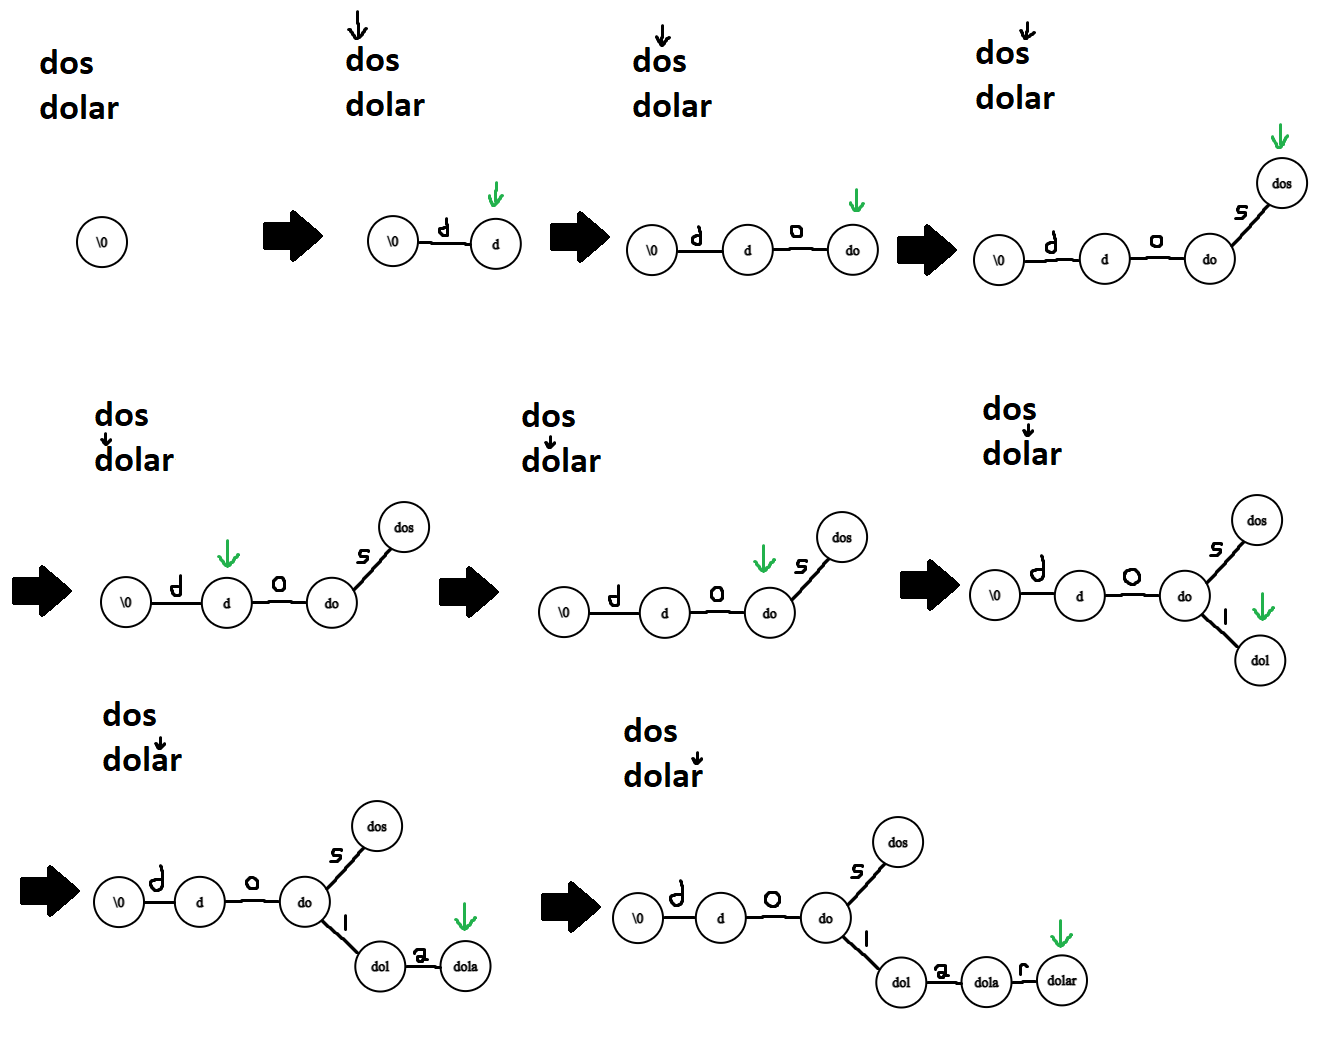
\includegraphics[scale=0.3]{Imagenes/construccion_arbol_dos_dolar.png}
\end{center}

El costo temporal de este metodo es $O(M)$, ya que se leen uno por uno los caracteres del diccionario.

\subsection*{Calculo de las transiciones de falla}
Dado un nodo $n$ que representa a un prefijo $p$, su transicion de falla apunta a aquel nodo que:

\begin{itemize}
    \item Representa al sufijo propio mas grande de $p$
    \item Si tiene como ancestro a una palabra aceptada del diccionario $x$, entonces el prefijo al que apunta
    su transición de falla no puede tener interseccíon con $x$.
\end{itemize}

Un primer intento para calcularlas seria asi: para cada nodo, recorrer el automata buscando una palabra
que cumpla estas condiciones, pero esto resulta muy costoso.

Esto se puede optimizar como sigue, suponiendo que quiero calcular
la transicion de falla de un nodo $N$. Asumiendo que todos los nodos que estan mas arriba que $N$ en el arbol
ya tienen transición de falla calculada. Se puede calcular la transición de $N$ de esta forma:

\begin{lstlisting}[language=C]
    // Voy hasta el padre de N y sigo su transicion de falla
    EstadoAutomata* estado = N->padre->transicionDeFalla;

    // El caracter que hay que usar para ir desde el padre de N hasta N
    char a = N->valorTransicionPadre;

    // Voy recorriendo las transiciones de falla hasta llegar hasta la raiz o hasta
    // que encuentre una transicion por a
    while (estado->padre != NULL && !estado_transicion_disponible(estado, a))
        estado = estado->transicionDeFalla;
    
    // Si hay una transicion por a, la sigo
    if (estado_transicion_disponible(estado, a))
        estado = estado->transicion[(int)a - 'a'];
    
    // El nodo hasta el que llegue es a donde apunta la transicion de falla de N
    N->transicionDeFalla = estado;
\end{lstlisting}

Esta manera requiere que las transiciones de falla de los ancestros de $N$ este calculada, asi que el algoritmo
final para calcular las transiciones de falla consiste en recorrer el arbol por niveles(usando BFS) y aplicar el algoritmo
de arriba.

\begin{lstlisting}[language=C]
    // Recorro el automata por niveles usando BFS y una cola
    // No es necesario crear copias del estado del automata, asi que
    // la funcion de copia es la identidad y la funcion destructora no hace
    // nada
    Cola colaEstados = cola_crear(copy_id, void_destroy);

    // Meto el estado inicial en la cola
    colaEstados = cola_push(colaEstados, estadoInicial);

    while (!cola_empty(colaEstados))
    {
        Automata estadoActual = (Automata)cola_front(colaEstados);
        colaEstados = cola_pop(colaEstados);

        // Si el estado actual es el inicial, tiene como padre al inicial o es un estado de aceptacion, su transicion de falla
        // apunta al estado inicial
        if (estadoActual == estadoInicial || estadoActual->padre == estadoInicial || estadoActual->palabraAceptada)
            estadoActual->transicionDeFalla = estadoInicial;
        else
        {
            // Voy hasta el padre del estadoActual y sigo su transicion de falla
            EstadoAutomata* estado = estadoActual->padre->transicionDeFalla;

            char valor_transicion = estadoActual->valorTransicionPadre;
            
            // Voy recorriendo las transiciones de falla hasta llegar hasta la raiz o hasta
            // que encuentre una transicion por c
            while (estado->padre != NULL && !estado_transicion_disponible(estado, valor_transicion))
                estado = estado->transicionDeFalla;
            
            // Si hay una transicion por a, la sigo
            if (estado_transicion_disponible(estado, valor_transicion))
                estado = estado->transicion[(int)valor_transicion - 'a'];
            
            // El nodo hasta el que llegue es a donde apunta la transicion de falla de N
            estadoActual->transicionDeFalla = estado;
        }   

        // Meto los estados que estan conectados por una transicion que no es de falla en la cola
        for (int i = 'a'; i <= 'z'; i++)
            if (estado_transicion_disponible(estadoActual, i))
                colaEstados = cola_push(colaEstados, estadoActual->transicion[i - 'a']);
    }
    cola_destroy(colaEstados);
\end{lstlisting}

Pareceria que el costo total en tiempo del algoritmo es del orden de $O(M^2)$, pero esto no es asi, en
total el costo es $O(M)$. 

Suponiendo que se quiere calcular las transiciones de falla para todos los prefijos de una palabra de largo
$h$. El proceso para calcular la transicion de falla de un nodo $v$ que esta en el nivel $k$ consiste en ir
hasta el padre de $v$, recorrer una cantidad $x$ de transiciones de falla desde ahi y luego seguir una transicion
extra hacia adelante(si es necesario). El nodo $u$ al que se llega haciendo estos pasos luego es unido a $v$ por
una transición de falla. La cantidad de transiciones de falla que se utilizan no puede ser mayor que $k$(dado que las
transiciones de falla "suben" en el arbol). Al pasar al nodo siguiente a $u$, la transicion de falla recien calculada
de $v$ evita recorrer nuevamente las $x$ transiciones del paso anterior. Gracias a esto, si se llego a un nodo por una
transición de falla, no se volvera a llegar a el de nuevo. Dado que la suma de las transiciones $x$ que se recorrieron
es menor al largo de las palabra $h$, la complejidad para una palabra no puede ser mas grande que $O(2h)$ y la complejidad
total para todo el diccionario es $O(2M) = O(M)$.

\subsection*{Calculo de las transiciones de salida}

El calculo de las transiciones de salida se puede hacer al mismo tiempo que el de las transiciones de falla. Luego de calcular
la transicion de falla de un nodo $v$ pueden pasar tres casos:

\begin{description}
    \item[La transición de falla de $v$ apunta a un nodo de aceptacion:] En este caso la transicion de salida apunta al mismo lugar.
    \item[La transicion de falla de $v$ apunta a un nodo $u$ con transicion de salida:] En este caso, la transición de salida de $v$ apunta al mismo
    lugar que el nodo de la transicion de salida de $u$.
    \item[Ninguno de los casos anteriores:] $v$ no tiene transicion de sallida.
\end{description}

Este calculo tiene un costo constante el tiempo.

El algoritmo final para calcular las transiciones de falla y de salida queda como sigue:

\begin{lstlisting}[language=C]
    // Recorro el automata por niveles usando BFS y una cola
    // No es necesario crear copias del estado del automata, asi que
    // la funcion de copia es la identidad y la funcion destructora no hace
    // nada
    Cola colaEstados = cola_crear(copy_id, void_destroy);

    // Meto el estado inicial en la cola
    colaEstados = cola_push(colaEstados, estadoInicial);

    while (!cola_empty(colaEstados))
    {
        Automata estadoActual = (Automata)cola_front(colaEstados);
        colaEstados = cola_pop(colaEstados);

        // Si el estado actual es el inicial, tiene como padre al inicial o es un estado de aceptacion, su transicion de falla
        // apunta al estado inicial
        if (estadoActual == estadoInicial || estadoActual->padre == estadoInicial || estadoActual->palabraAceptada)
            estadoActual->transicionDeFalla = estadoInicial;
        else
        {
            // Voy hasta el padre del estadoActual y sigo su transicion de falla
            EstadoAutomata* estado = estadoActual->padre->transicionDeFalla;

            char valor_transicion = estadoActual->valorTransicionPadre;
            
            // Voy recorriendo las transiciones de falla hasta llegar hasta la raiz o hasta
            // que encuentre una transicion por c
            while (estado->padre != NULL && !estado_transicion_disponible(estado, valor_transicion))
                estado = estado->transicionDeFalla;
            
            // Si hay una transicion por a, la sigo
            if (estado_transicion_disponible(estado, valor_transicion))
                estado = estado->transicion[(int)valor_transicion - 'a'];
            
            // El nodo hasta el que llegue es a donde apunta la transicion de falla de N
            estadoActual->transicionDeFalla = estado;
        }
        
        // Calculo la transicion de salida
        if (estadoActual->transicionDeFalla->palabraAceptada)
            estadoActual->transicionDeSalida = estadoActual->transicionDeFalla;
        else
            estadoActual->transicionDeSalida = estadoActual->transicionDeFalla->transicionDeSalida;

        // Meto los estados que estan conectados por una transicion que no es de falla en la cola
        for (int i = 'a'; i <= 'z'; i++)
            if (estado_transicion_disponible(estadoActual, i))
                colaEstados = cola_push(colaEstados, estadoActual->transicion[i - 'a']);
    }
    cola_destroy(colaEstados);
\end{lstlisting}

\subsection*{Complejidad final}

Sea:
\begin{itemize}
    \item $N$ el largo de una frase a procesar
    \item $M$ la longitud total de todas las palabras del diccionario
    \item $k$ el largo de la palabra mas larga del diccionario
    \item $Z$ la cantidad de ocurrencias de las palabras del diccionario en la frase
\end{itemize}

La complejidad temporal de crear el automata termina siendo $O(M)$.
La complejidad espacial de crear el automata termina siendo $O(M \cdot 26) = O(M)$.

La complejidad temporal de espaciar una frase es $O(N+Z \cdot \log Z)$.
La complejidad espacial de espaciar una frase es $O(k+Z)$

La complejidad temporal total del algoritmo es $O(N+M+Z\cdot \log Z)$ y la complejidad espacial es
$O(k+M+Z)$.




\end{document}